%\documentclass{cumcmthesis}
\documentclass[withoutpreface,bwprint]{cumcmthesis} %去掉封面与编号页
\title{}
\tihao{A} % 题号
\baominghao{4321} % 报名号
\schoolname{湘潭大学}
\membera{米科润}
\memberb{李云潇}
\memberc{周昕阳}
\supervisor{杨柳}
\yearinput{2021} % 年
\monthinput{09} % 月
\dayinput{12} % 日
\bibliographystyle{plain}
\makeatletter
\newlength\savefboxrule
\newlength\savefboxsep
\edef\example@name{\jobname-example.aux}
\newenvironment{hexample}%
{%
\renewcommand{\minted@FVB@VerbatimOut}[1]{%
  \@bsphack
  \begingroup
    \FV@DefineWhiteSpace
    \def\FV@Space{\space}%
    \FV@DefineTabOut
    \let\FV@ProcessLine\minted@write@detok
    \immediate\openout\FV@OutFile ##1\relax
    \let\FV@FontScanPrep\relax
    \let\@noligs\relax
    \FV@Scan}
\minted@FVB@VerbatimOut{\example@name}}%
{\minted@FVE@VerbatimOut%
  \trivlist\item\relax
  \setlength{\savefboxrule}{\fboxrule}%
  \setlength{\savefboxsep}{\fboxsep}%
  \setlength{\fboxsep}{0.015\textwidth}%
  \setlength{\fboxrule}{0.4pt}%
  \fcolorbox[gray]{0}{0.95}{%
    \begin{minipage}[c]{1\textwidth}%
          \setlength{\fboxrule}{\savefboxrule}%
          \setlength{\fboxsep}{\savefboxsep}%
          \setlength{\parskip}{1ex plus 0.4ex minus 0.2ex}%
          \normalsize\input{\example@name}%
        \end{minipage}%
  }%
  \hfill%
  %\fbox{%
   % \begin{minipage}[c]{0.45\textwidth}%
   %   \setlength{\fboxrule}{\savefboxrule}%
   %   \setlength{\fboxsep}{\savefboxsep}%
   %   \setlength{\parskip}{1ex plus 0.4ex minus 0.2ex}%
   %   \normalsize\input{\example@name}%
   % \end{minipage}%
  %}%
  \endtrivlist
}
\newenvironment{vexample}%
{%
\renewcommand{\minted@FVB@VerbatimOut}[1]{%
  \@bsphack
  \begingroup
    \FV@DefineWhiteSpace
    \def\FV@Space{\space}%
    \FV@DefineTabOut
    \let\FV@ProcessLine\minted@write@detok
    \immediate\openout\FV@OutFile ##1\relax
    \let\FV@FontScanPrep\relax
    \let\@noligs\relax
    \FV@Scan}
\minted@FVB@VerbatimOut{\example@name}}%
{\minted@FVE@VerbatimOut%
  \trivlist\item\relax
  \setlength{\savefboxrule}{\fboxrule}%
  \setlength{\savefboxsep}{\fboxsep}%
  \setlength{\fboxsep}{0.015\textwidth}%
  \setlength{\fboxrule}{0.4pt}%
  \begin{minipage}[c]{\textwidth}
  \fcolorbox[gray]{0}{0.95}{%
    \begin{minipage}[c]{\textwidth-0.03\textwidth-0.8pt}%
      \setlength{\fboxrule}{\savefboxrule}%
      \setlength{\fboxsep}{\savefboxsep}%
      \small\inputminted[breakanywhere,breaklines=true,numbers=left]{latex}{\example@name}%
    \end{minipage}%
  }\\
  \fbox{%
    \begin{minipage}[c]{\textwidth-0.03\textwidth-0.8pt}%
      \setlength{\fboxrule}{\savefboxrule}%
      \setlength{\fboxsep}{\savefboxsep}%
      \setlength{\parskip}{1ex plus 0.4ex minus 0.2ex}%
      \normalsize\input{\example@name}%
    \end{minipage}%
  }%
  \end{minipage}
  \endtrivlist
}
\newenvironment{floatexample}%
{%
\renewcommand{\minted@FVB@VerbatimOut}[1]{%
  \@bsphack
  \begingroup
    \FV@DefineWhiteSpace
    \def\FV@Space{\space}%
    \FV@DefineTabOut
    \let\FV@ProcessLine\minted@write@detok
    \immediate\openout\FV@OutFile ##1\relax
    \let\FV@FontScanPrep\relax
    \let\@noligs\relax
    \FV@Scan}
\minted@FVB@VerbatimOut{\example@name}}%
{\minted@FVE@VerbatimOut%
  \trivlist\item\relax
  \setlength{\savefboxrule}{\fboxrule}%
  \setlength{\savefboxsep}{\fboxsep}%
  \setlength{\fboxsep}{0.015\textwidth}%
  \setlength{\fboxrule}{0.4pt}%
  \fcolorbox[gray]{0}{0.95}{%
    \begin{minipage}[c]{\textwidth-0.03\textwidth-0.8pt}%
      \setlength{\fboxrule}{\savefboxrule}%
      \setlength{\fboxsep}{\savefboxsep}%
      \small\inputminted[breakanywhere,breaklines=true,numbers=left]{latex}{\example@name}%
    \end{minipage}%
  }\\
  \input{\example@name}%
  \endtrivlist
}
\makeatother




\begin{document}
	\maketitle
	\begin{abstract}
粮食是国家的战略物质,是人民的生活必需品,是粮农的重要经济来源,同时也是很多工业产品的原料。本文研究影响粮食种植面积的指标体系,讨论粮食最低收购价政策,建立关于粮食最低收购价的数学模型,并给出调控粮食种植的优化决策和建议,具有重要的理论与现实意义。\par
针对问题一,首先选取农业劳动力人口、农民人均受教育程度、城乡收入差距等11个影响粮食种植面积的候选因素,然后利用Spearman相关检验法通过SPSS对湖南省和辽宁省的水稻影响其种植面积的指标与其种植面积进行相关性检验,得到影响因素的指标体系,其中影响湖南省和辽宁省水稻种植面积的指标中具有相关关系的指标分别有6个和7个。最后,利用所选取水稻种植面积相关的指标为自变量,以水稻的种植面积为因变量运用主成分回归分析分别建立模型,检验后发现模型具有较好的拟合结果。\par
针对问题二,根据粮食区域的差异与问题一中建立的指标体系,本文运用主成分-协方差分析方法分别对湖南省与辽宁省的水稻进行粮食最低收购价政策执行效果的评价。为了消除变量间的共线性,对指标体系其他变量进行主成分分析,根据累计方差贡献率选取前几个主成分并作为协变量建立粮食最低收购价政策与粮食种植面积的协方差分析模型。经过计算得出:粮食最低收购价政策对辽宁水稻种植面积有显著的影响并且政策实行后,辽宁省的水稻种植面积有了大幅的增加,但粮食最低收购价对湖南水稻种植面积无显著影响。\par
针对问题三,首先选取影响我国水稻价格、供给量及需求量的指标。然后基于供需理论构建粮食供需及价格联动模型,即水稻的供给模型、需求模型和价格模型,并运用广义矩估计法通过Stata对模型进行估计最终得到水稻价格体系模型。\par
针对问题四,在问题三供需价格联动模型的基础上进行优化,将粮食种植面积最大作为优化模型目标函数,从种植面积、财政支出及库存量三个方面进行约束。得到水稻合理定价模型,应用该模型对国家“十二五”时期公布的粮食最低收购价进行评价。定义误差率做为粮食最低收购价的评价标准,通过Matlab计算结果可以看出2012、2013年公布的粮食最低收购价格较为合理。最后应用无偏GM(1,1)模型对2017 年粮食最低收购价进行预测,得出水稻最低收购价格预测结果为152。\par
针对问题五,在问题四中水稻的合理定价模型的基础上进行优化。在原有模型的基
础上,固定其它变量不变,将种植面积提高5\%,在满足约束条件的基础上,利用Matlab计算得出调整后的粮食最低收购价为153元。\par
对于问题六,根据问题一到问题五所得到的结论,本文从影响粮食种植面积因素、粮食最低收购价政策实施、粮食价格规律及粮食最低收购价制定四个方面给出相应的调控粮食种植的优化决策和建议。\par
	\keywords{种植面积\quad 收购价政策\quad 价格体系模型\quad 主成分分析\quad}
	\end{abstract}



	\section{问题重述}
	\subsection{问题背景}
粮食不仅是人们日常生活中必不可少的食物,也是维护国家经济发展和政治稳定的战略物资,具有不可替代的特点。中国的粮食产业正面临着潜在的风险,因此研究我国粮食保护政策的作用和意义非常重要。\par
粮食最低收购价政策属于粮食保护政策体系,一般来说,中国的粮食收购价格由市场供求关系决定,国家在充分发挥市场机制作用的基础上实行宏观调控。为保护农民利益,保证粮食市场供应,国家在粮食主产区对重点粮食品种实行最低收购价政策,公布最低收购价后,在最低收购价政策执行期间,当市场上粮食的实际收购价格低于国家确定的最低收购价时,国家委托符合一定条件的粮食企业按国家确定的最低收购价收购农民种植的粮食,以保护种粮农民的积极性。中国自2005年起对粮食主产区实行最低收购价政策,并连续多年提高最低收购价价格,粮食最低收购价政策已成为国家保护粮食生产的最重要举措之一。\par
也有学者不同意这种最低收购价政策,认为粮食的实际收购价格即粮食的市场收购价格应该由粮食的供求双方通过市场调节来决定。作为一项粮食种植保护政策,最低收购价政策扭曲了粮食市场的供求行为,即该政策的实施容易抬高市场收购价格,导致粮食企业承担很大的经营风险。\par
同时,学者们对粮食最低收购价政策实施效果的评价也有不同意见:在一些地区,某些粮食品种的种植面积和粮食总产量不增反减,这使一些学者对粮食最低收购价政策的效果产生了质疑;但也有一些学者认为如果不实行粮食最低收购价政策,这些地区某些粮食品种的种植面积可能会下降得更快,因而认为粮食最低收购价政策对稳定或增加粮食种植面积有积极作用。\par
粮食种植面积是决定粮食供给的关键因素,也是保障粮食安全的重要前提。衡量粮食最低收购价政策的实施效果,主要是比较政策实施前后粮食种植面积是否有明显变化,但影响粮食种植面积的因素很多,研究粮食最低收购价政策的实施效果,不能只根据种植面积的变化来评估\par
同时,也有学者讨论了粮食最低收购价设定的合理范围,他们指出,最低收购价不是实际的市场收购价,而是一种心理安慰价,是收购粮食的底价,种粮农民决定是否种粮,主要取决于种粮获得的纯收入的大小。\par
过高的粮食最低收购价不仅会抬高粮食的市场价格,从而增加消费者的负担,而且还会增加粮食库存的压力和国家财政支出的风险。另一方面,过低的最低收购价会抑制农民种粮的积极性,造成粮食种植面积的萎缩,这也是国家不愿意看到的。




	
	
	
	\subsection{问题的提出}
\begin{enumerate}[itemsep=0pt,parsep=0pt,label=(\arabic*)]
\item 影响粮食种植面积的因素很多,它们之间的关系很复杂,可能存在粮食品种和地区差异。建立影响粮食种植面积的指标体系和有关粮食种植面积的数学模型,讨论和评价指标体系的合理性,研究它们之间的关系,并对得到的相应结果的可信度和可靠性进行检验和分析。
\item 建立粮食最低收购价政策实施效果的评价模型。并利用建立的评价模型,在考虑粮食品种和地区差异的情况下,选择几个省份对粮食主产区的粮食最低收购价执行效果进行比较研究。
\item 粮食市场收购价是粮食企业收购粮食的市场价格,是由粮食供求双方通过市场调节决定的。它与粮食最低收购价一起构成了粮食价格体系,是宏观价格调控体系中具有一定相对独立性的重要措施。利用数据分析或建立数学模型,探讨中国粮食价格的特殊规律性。
\item 请结合前期研究和国家最低收购价政策的初衷,建立粮食最低收购价的合理定价模型,评估 "十二五 "期间国家发改委公布的最低收购价的合理性,并利用该模型预测2017年粮食最低收购价的合理区间。
\item 与2000年相比,2015年中国的小麦播种面积略有下降。如果国家希望增加$5\%$的小麦种植面积,是否可以通过调整粮食最低收购价来实现?请说明理由。
\item 根据你们的研究结果,提出规范粮食种植的最佳决策和建议。
\end{enumerate}






\section{问题分析}
问题一要求建立影响粮食种植面积的指标体系和有关粮食种植面积的数学模型,讨论指标体系的合理性及他们之间的关系,并对得出的相应结果的可信度和可靠性给出检验和分析。这首先要求我们对粮食(水稻)种植区域进行划分,从划分的区域中选出代表性的省份分别进行研究,然后选取影响粮食种植面积的候选因素,并用Spearman相关检验的方法分别进行相关性检验,最终选取代表省份中与种植面积相关的因素,最后以上述指标为自变量,各省份水稻种植面积为因变量进行主成分回归分析。\par
问题二要求衡量粮食最低收购价政策实施的效果,主要是比较政策实施前后粮食种植面积是否发生了显著性的变化,传统的方差分析法并不能排除掉其他可能影响种植面积的因素的干扰,要求我们采用协方差分析的方法来判断粮食最低收购价政策的有效性。另一方面,为消除各个因素之间存在的显著关系,进行协方差分析之前,首先要对各个变量进行主成分分析。\par
对于问题三,要运用数据分析或建立数学模型探讨我国粮食价格所具有的特殊规律性。这要求我们首先选取影响我国水稻价格、供给量及需求量的指标。然后基于供需理论构建粮食供需及价格联动模型。即对水稻的供给模型、需求模型和价格模型,并运用广义矩估计法对该模型进行估计。\par
对于问题四,建立粮食最低收购价的合理定价模型,进而评价对“十二五”期间国家发展与改革委员会公布的粮食最低收购价价格,并对2017年的粮食最低收购价的合理范围进行预测。要求我们首先在问题三供需价格联动模型的基础上进行优化,将粮食种植面积最大作为优化模型目标函数,从种植面积、财政支出及库存量三个方面进行约束。分别得到水稻的合理定价模型;然后应用所建立的水稻合理定价模型对国家“十二五”时期公布的粮食最低收购价进行评价。定义误差率做为粮食最低收购价的评价标准计算结果判断公布的粮食最低收购价格的合理性。最后应用所建立的模型对2017年粮食最低收购价进行预测,得出水稻最低收购价格预测区间。\par
对于问题五,要求通过调整粮食最低收购价使我国小麦种植面积增加$5\%$。由于前文仅讨论水稻情况,我们将对水稻进行分析。我们将在问题四中水稻的合理定价模型的基础上进行优化。在原有模型的基础上,固定其它变量不变,将种植面积提高5\%。在满足约束条件的基础上,利用计算得出调整后的粮食最低收购价。	
对于问题六,要求根据研究结论,提出调控粮食种植的优化决策和建议。本问题我们将根据问题一到问题五所得到的结论,从影响粮食种植面积因素、粮食最低收购价政策实施、粮食价格规律及粮食最低收购价制定四个方面给出相应的调控粮食种植的优化决策和建议。
	
	\section{模型的假设}
	\begin{itemize}
	\item 不考虑制度变迁、政策等的变化
	\item 不考虑除文章选取因素外其他因素影响
	\item 不考虑水稻品种的差异
	\item 国内市场是完全竞争的,粮食价格完全由市场决定
	\item 假设粮食种植面积的显著变化与否,可以衡量粮食最低收购价政策的实施效
	果
	\end{itemize}\par	
	
	
	
	
	
	\newpage
	\section{符号说明}
	\begin{table}[!htbp]
		\centering
		\label{tabfuhao}
		\setlength\tabcolsep{20pt}%设置列间距
		\begin{tabular}{cccc}
		\toprule[1.5pt]
		符号 & 说明 & 符号 & 说明 \\
		\midrule[1pt]
	$\rho$ & Spearman相关系数 & $x_1$ &农业劳动力人口 \\
	$x_2$ & 农民受教育程度 & $x_3$ &城乡收入差距\\
	$x_4$ & 家庭负担 & $x_5$ & 水稻市场价\\
	$x_6$ & 水稻成本 & $x_7$ & 水稻相对收益竞争力\\
	$x_8$ & 总播种面积 & $x_9$ & 受灾情况 \\
	$x_{10}$ & 粮食的净出口 & $x_{11}$ & 城市化水平\\
	$y_1$ & 湖南省水稻播种面积 & $y_2$ &辽宁省水稻播种面积\\
	$G_t^s$&t时期供给量&$P_{t}$&$t$时期价格水平\\
	$IM_t$&t时期进口量&$U_p^t$&t时期单产水平\\
	$PR_t$&t时期种植面积&$CU_t$&t时期居民消费水平\\
	$URBAN_t$&t时期城镇化水平&$IN_t$&t时期进口水平\\
	$SP_t$&替代品价格&$EX_t$&t时期出口水平\\
	$PO_t$&最低粮食收购价&$\lambda_0-\lambda_5$&粮食供给模型系数\\
	$\alpha_{0}-\alpha_{5}$&粮食需求模型参数&$\beta_{0}-\beta_{6}$&粮食价格模型参数\\
		\bottomrule[1.5pt]
		\end{tabular}
	\end{table}
$x_1-x_{11}$为两省各自数据
	




	











	
		\section{问题一:粮食种植面积的指标体系模型的建立}
		\subsection{模型的建立与求解}
		\subsubsection{指标选取}
粮食的种植面积是决定粮食供给的关键因素,也是保障粮食安全的重要
前提。衡量粮食最低收购价政策实施的效果,主要是比较政策实施前后粮食种植面积是否有显著性变化。我国自2005年起开始对粮食主产区实行了最低收购价政策。故选取1995-2014 时间段内的数据,即实行政策前后共20 年的数据进行研究。\par
水稻种植面积在我国约占粮食作物面积的30%,同时水稻主产区中的东北平原区和长江流域区中辽宁和湖南为水稻种植的代表性省份。\par
本文选择水稻在辽宁和湖南两省影响其种植面积的农业劳动力人口、农民人均受教育程度、城乡收入差距、农民家庭负担、水稻市场价格、水稻生产成本、水稻相对收益竞争力、农作物总播种面积、受灾情况、我国粮食净出口量、城市化水平这11个指标进行分析,表\ref{tab:ln}是辽宁省上述指标的部分数据\footnote{详细数据及解释见支撑材料}。
\begin{table}[htbp]
  	\caption{辽宁省指标}
  	\centering
  	\label{tab:ln}
	\begin{tabular}{cccc}
    \toprule[2pt]
    水稻播种面积 & 农业劳动力人口& 城乡收入差距 & 水稻市场价\\
    \midrule[1.5pt]
    4457.50 & 2071.61 & 3.30  & 82.40 \\
    4458.34 & 1994.90 & 2.80  & 74.29 \\
    4470.35 & 1998.59 & 2.60  & 68.22 \\
    4395.23 & 2002.51 & 2.60  & 51.49 \\
    4444.27 & 2026.09 & 2.70  & 55.21 \\
    \ldots  & \ldots  &\ldots &\ldots \\
    4464.86 & 1690.03 & 2.90  &119.45 \\
    4559.03 & 1679.94 & 2.90  &133.20 \\
    4619.41 & 1668.99 & 2.90  &130.84 \\
    4631.01 & 1656.01 & 2.70  &127.03 \\
    4690.33 & 1651.37 & 2.60  &130.49 \\
    \bottomrule[2pt]
    \end{tabular}%
\end{table}

\subsubsection{Spearman相关检验}
斯皮尔曼(Spearman)相关系数属于非参数统计方法,是描述两组变量之间是否存在着相同或相反趋同性的一种指标,对原始变量的分布不作要求,仅需要确定变量在每个点(时期)上的等级即可获得,因此具有较好的性质,适用范围较广。对于样本容量为n的样本,n个原始数据$ X_{i},Y_{i}$被转换成等级数据$ x_{i},y_{i}$,相关系数$\rho$为:
\begin{equation*}
\rho=\frac{\sum_{i}\left(x_{i}-\bar{x}\right)\left(y_{i}-\bar{y}\right)}{\sqrt{\sum_{i}\left(x_{i}-\bar{x}\right)^{2} \sum_{i}\left(y_{i}-\bar{y}\right)^{2}}}
\end{equation*}
,其中等级数据$x_{i},y_{i}$是每个原始数据的降序位置的平均\upcite{斯皮尔曼等级相关系数}。\par
当以样本的数据来推测总体时,由于样本带有随机性,在小样本时数据间有相关,但总体之间不一定相关。因此有必要进行假设检验。在此,设定原假设$H_0$研究的总体之间无相关,备责假设$H_1$为研究的总体之间相关。用$\rho$的分布来检验X与Y是否独立。当n较大时$\sqrt{n-1} r_{s}$的近似分布为$N(0,1)$,由此构造拒绝域和计算相应的t检验值,当t检验值值小于某一显著水平(本文规定0.05)时,则拒绝原假设。
\begin{figure}[!h]
    \centering
    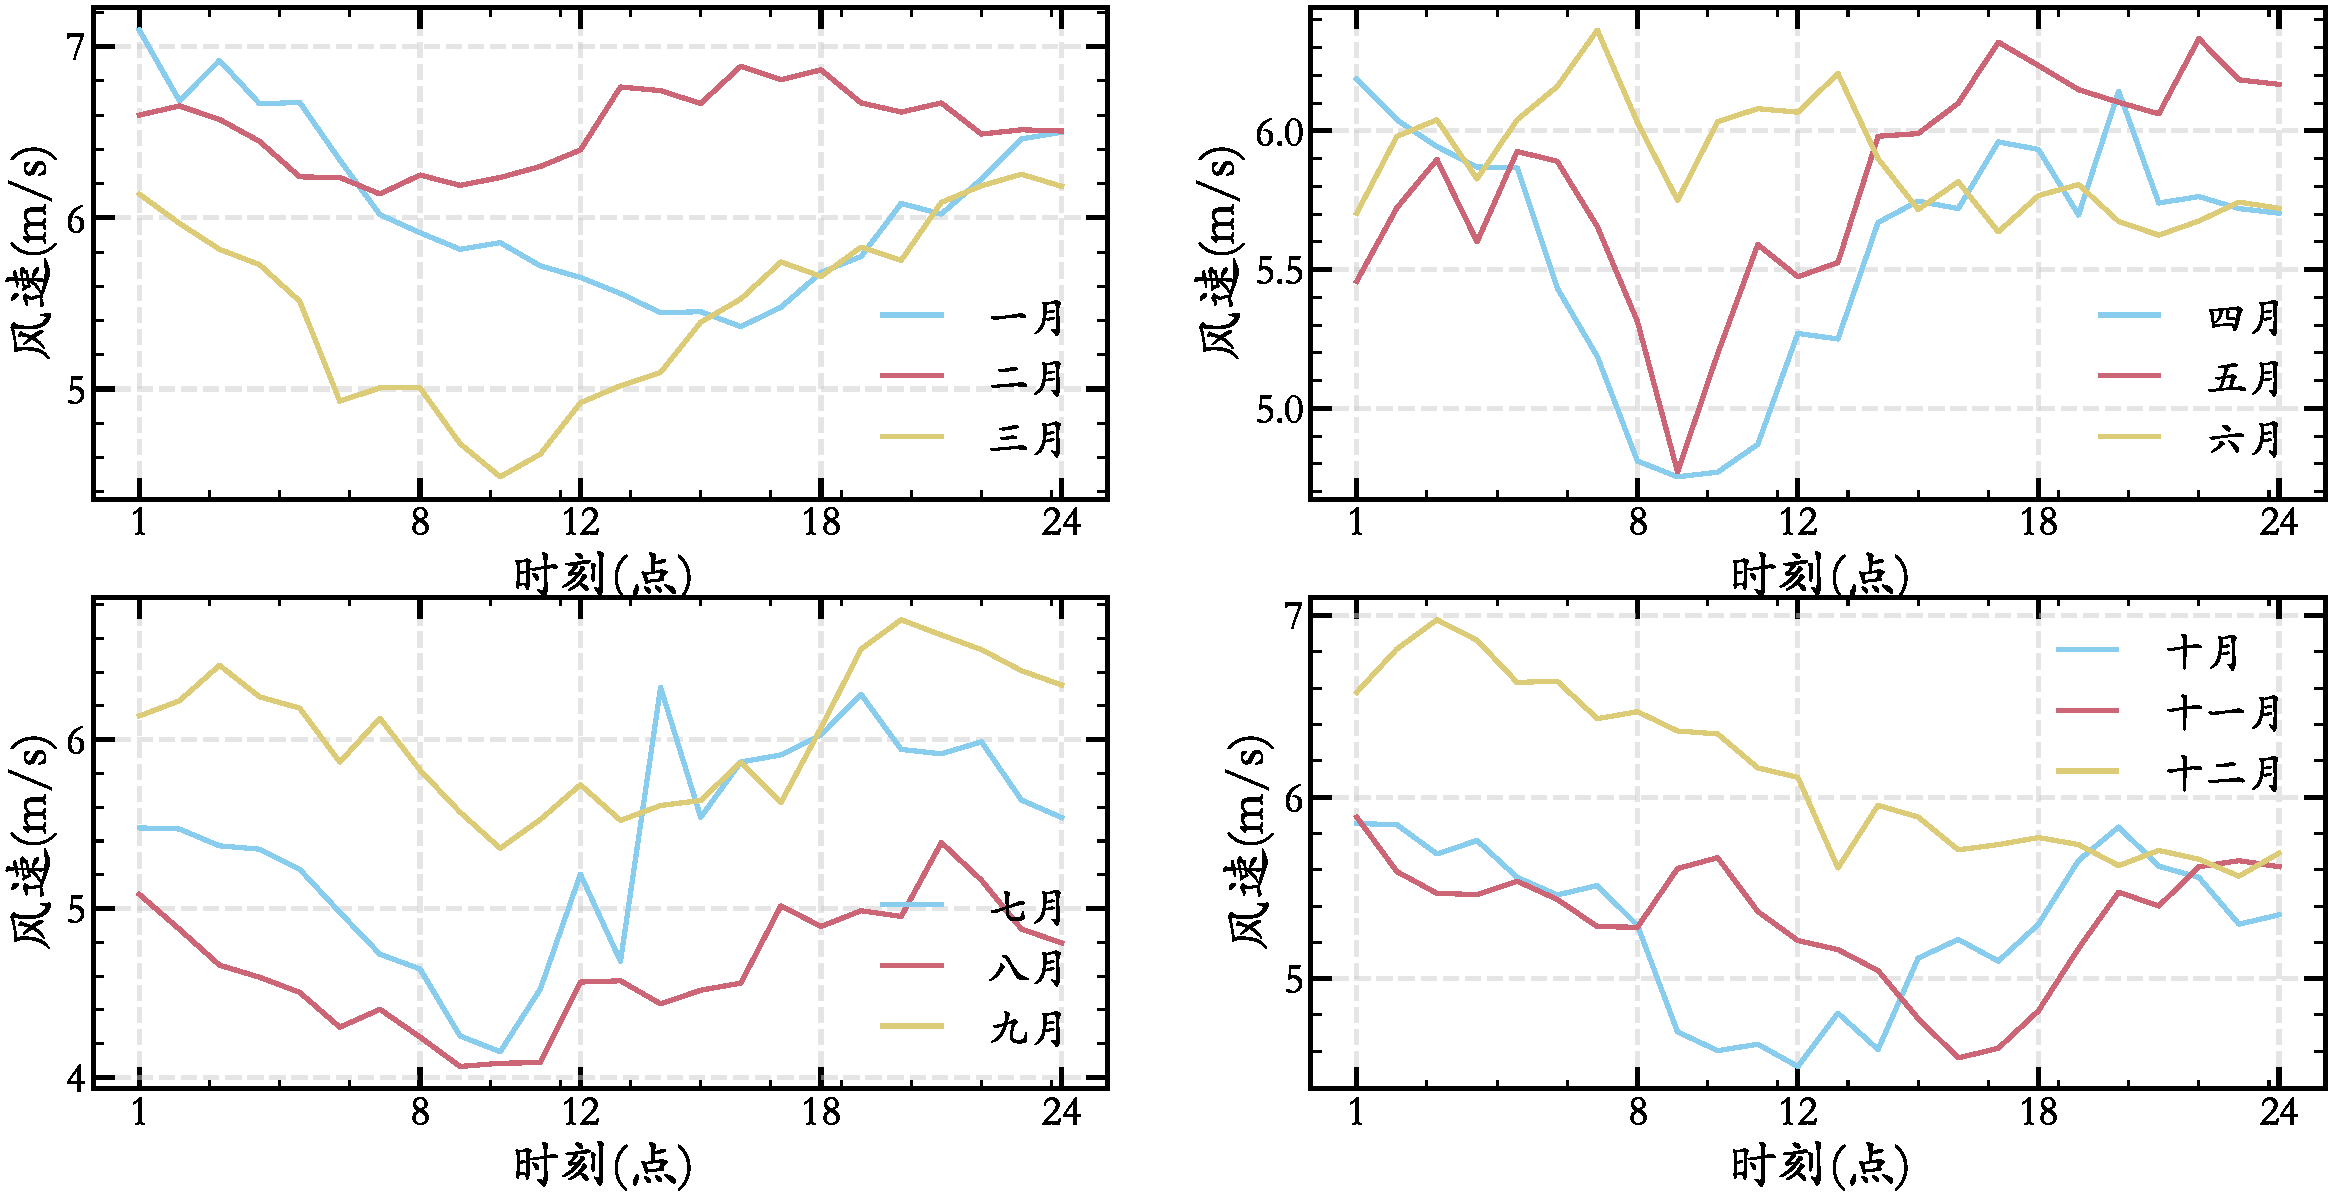
\includegraphics[width=0.935\textwidth]{fig1}
    \caption{湖南相关系数热力图}
    \label{fig:sp1}
\end{figure}\par
利用SPSS得到,图\ref{fig:sp1}是经过显著水平0.05筛选后的湖南Spearman相关系数热力图,由图见得,农民受教育程度、家庭负担、受灾情况、相对收益竞争力和城市化水平是无关联的指标,于是我们剔除掉这些指标。\par
\begin{figure}[!h]
    \centering
    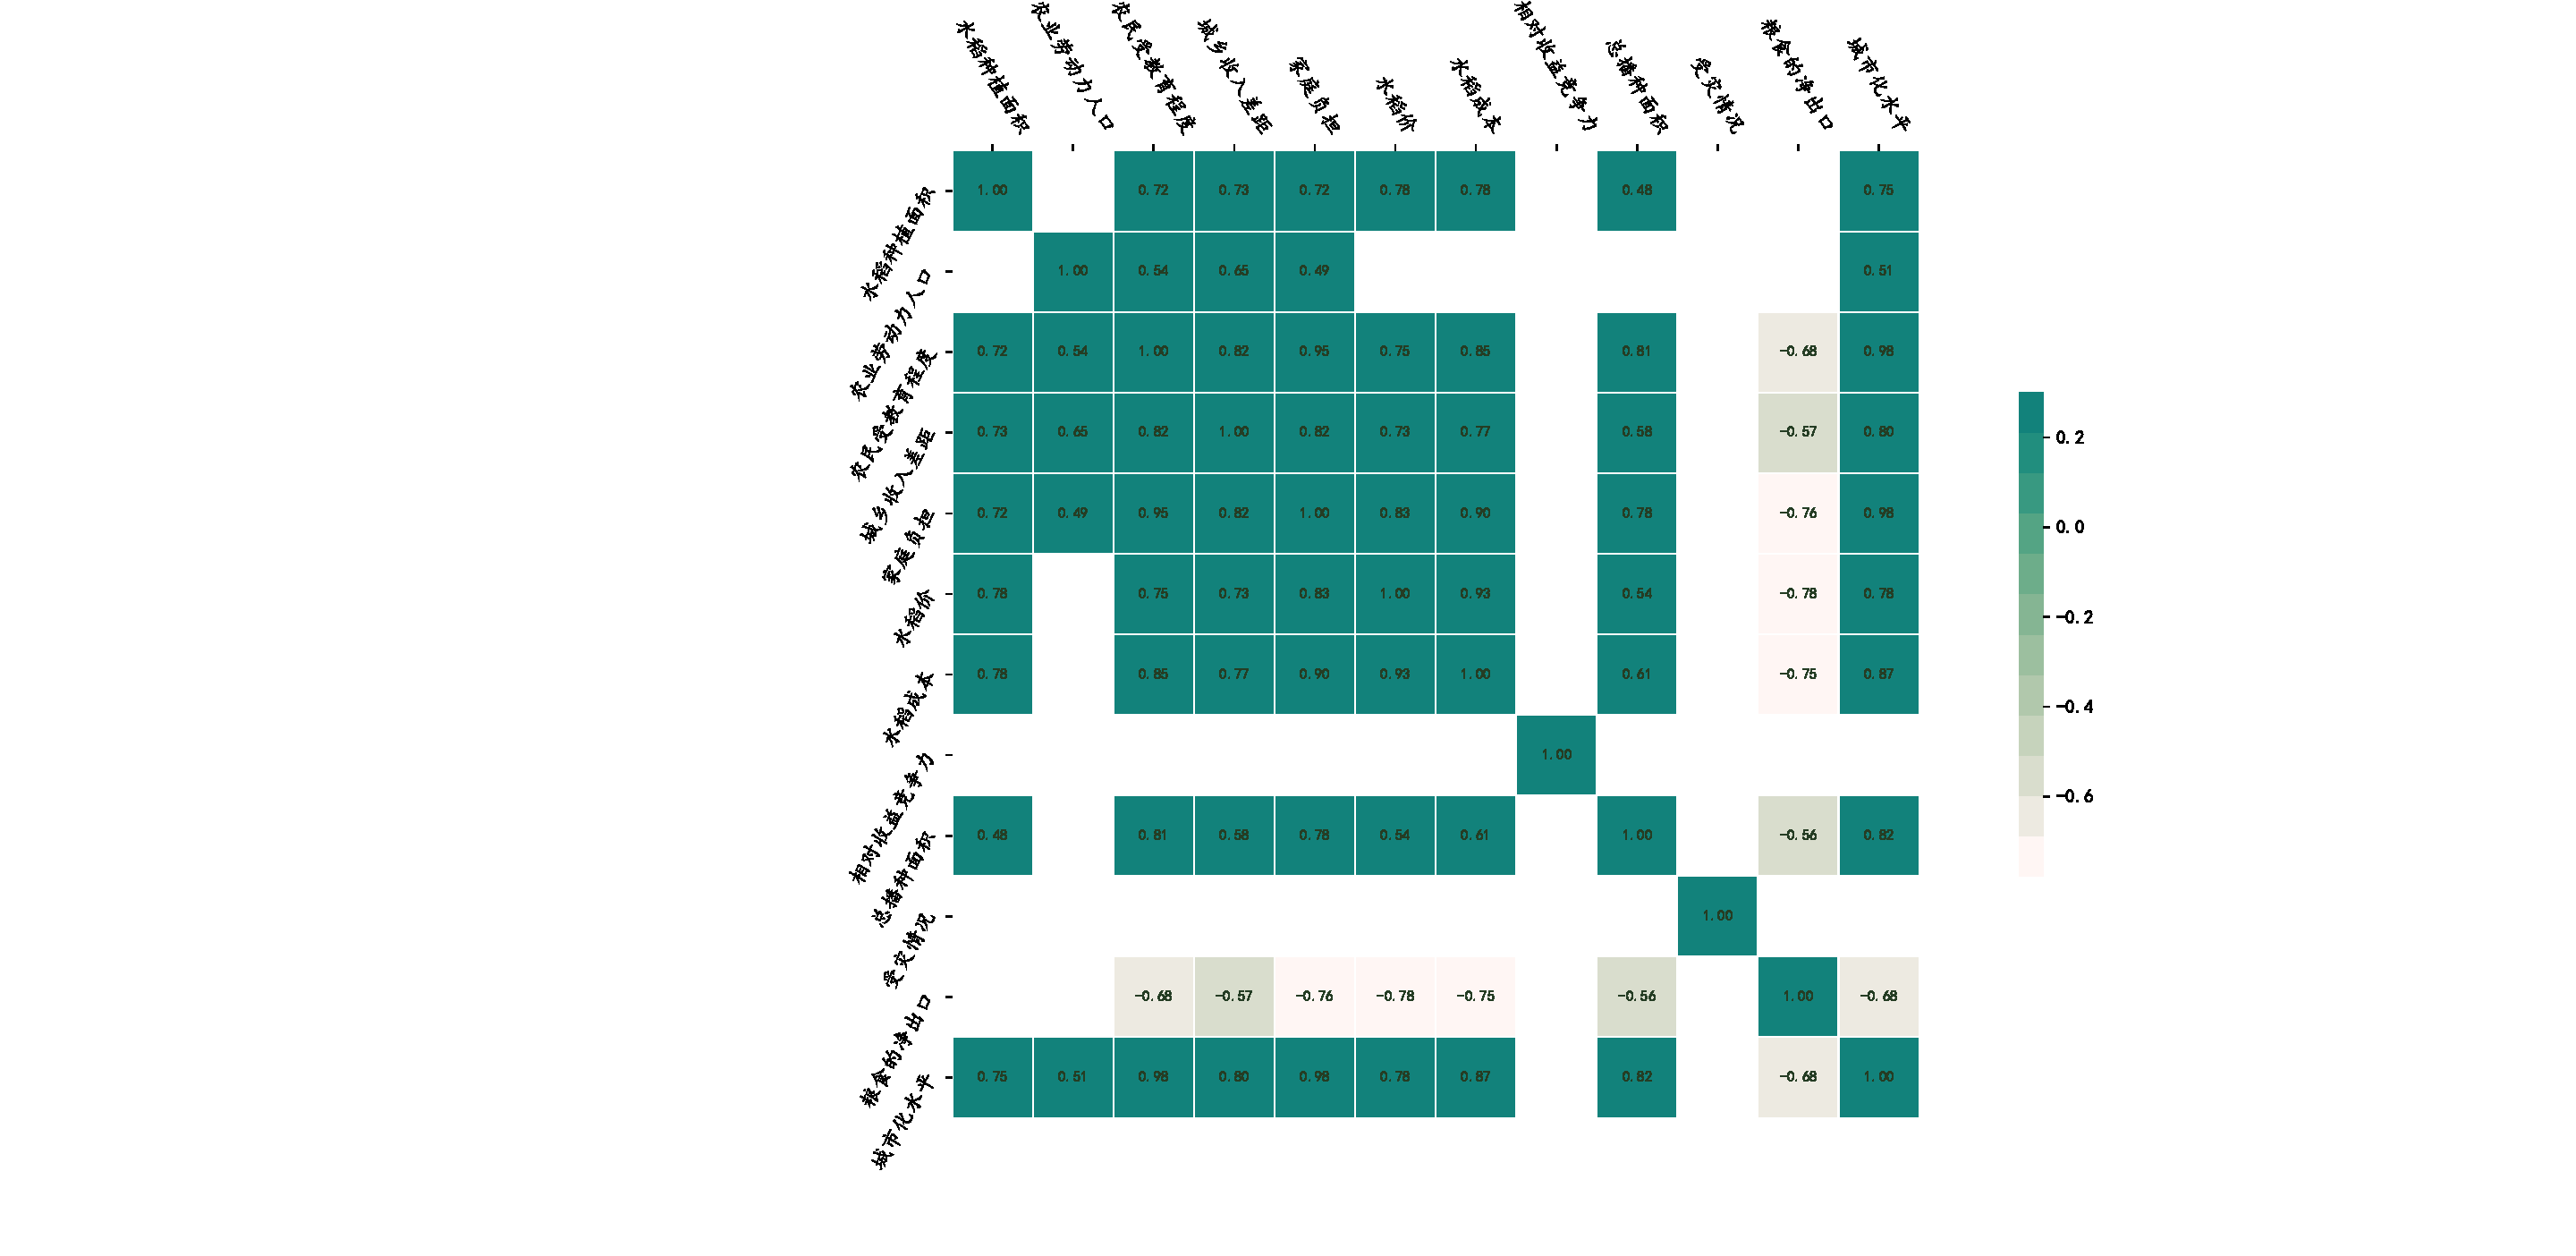
\includegraphics[width=0.935\textwidth]{fig2}
    \caption{辽宁相关系数热力图}
    \label{fig:sp2}
\end{figure}\par
图\ref{fig:sp2}是经过显著水平0.05筛选后的辽宁Spearman相关系数热力图,同理,我们剔除农业劳动力人口、相对收益竞争力、受灾情况、粮食净出口这些无关联指标。\par
\subsubsection{主成分回归分析}
主成分回归分析是为了克服最小二乘((LS)估计在数据矩阵 存在多重共线性时表现出的不稳定性而提出的,采用的方法是将原来的回归自变量变换到另一组变量,即主成分,选择其中一部分重要的主成分作为新的自变量,丢弃了一部分影响不大的自变量,实际上达到了降维的目的,然后用最小二乘法对选取主成分后的模型参数进行估计,最后再变换回原来的模型求出参数的估计\upcite{数学建模算法与应用}。\par
根据前文中选取的两省份指标,以辽宁省为例,我们利用Matlab对其进行主成分回归分析,步骤如公式(\ref{con:cha})所在表格:\par
\begin{hexample}
\begin{enumerate}
\item 数据标准化后得到相关系数矩阵
\item 得到相关系数矩阵的特征值贡献率为:$83.3\%,91.9\%,96.4\%,98.6\%,99.5\%,99.8\%,100\%$
\item 选取前四个主成分:$z_1.z_2,z_3,z_4$
\item 令水稻种植面积为因变量、$z_1.z_2,z_3,z_4$为自变量进行回归分析,得到:$y=0.3089z_1+0.2047z_2+0.6498z_3-0.6224z_4$(由于数据标准化,回归方程常数项为1)
\item 恢复到原始自变量,表达式为\\
\begin{equation}
\label{con:cha}
\begin{split}
y_2=&784.4475+89.5086x_2+39.9069x_3+0.0027x_4+1.1605x_5\\
&+1.1031x_6-0.3393x_8+1.5122x_{11}
\end{split}
\end{equation}
\item 计算得出回归方程剩余标准差为47.8944
\end{enumerate}
\end{hexample}
		
\subsection{模型的结果分析}
由上文,我们通过Spearman讨论了指标体系的合理性并筛选出两省中与水稻种植面积相关的指标。其中,湖南省的指标为农业劳动力人口、城乡收入差距、水稻市场价、水稻成本、总播种面积、受灾情况;辽宁省的指标为农民受教育程度、城乡收入差距、家庭负担、水稻市场价、水稻成本、总播种面积。
利用主成分回归分析,除得到辽宁省各指标与水稻种植面积的关系函数外,同理我们得到了湖南省各指标与水稻种植面积的回归函数(选取四个主成分,回归方程剩余标准差为147.1404):
\begin{equation*}
\begin{split}
y_1=&2927.194118-0.064138x_1-151.362909x_3+1.307020x_5+1.461505x_6\\
&+0.238906x_8-279.629816x_9
\end{split}
\end{equation*}\par

		
		
		
		
	
		\section{问题二:最低收购价效果评估模型}
		%\subsection{模型的建立}
		\subsection{主成分分析降维}
以湖南省为例,对通过spearman 相关性检验的6个变量进行主成分分析,结果如表\ref{tab:hnfc}:\par
		\begin{table}[htbp]
		  \centering
		  \caption{湖南省主成分方差贡献表}
		    \begin{tabular}{cccc}
		    \toprule[2pt]
		   &特征值 & 方差贡献率 & 累计贡献率\\
		    \midrule[1.5pt]
		  1 & 3.410502 & 0.568417 & 0.568417 \\
		  2 & 1.551153 & 0.258526 & 0.826943 \\
		  3 & 0.619561 & 0.10326 & 0.930203 \\
		  4 & 0.32531 & 0.054218 & 0.984421 \\
		  5 & 0.057284 & 0.009547 & 0.993968 \\
		  6 & 0.036189 & 0.006032 & 1 \\
		    \bottomrule[2pt]
		    \end{tabular}%
		  \label{tab:hnfc}%
		\end{table}%
可见前三个主成分的累计贡献率达到了$93.02\%$,即前两个主成分所包含的信息占全部信息的$93.02\%$,因此选择前三个主成分即可。各变量在前两个主成分中的系数见表\ref{tab:blxs}。\par
		\begin{table}[htbp]
		  \centering
		  \caption{各变量的系数}
		    \begin{tabular}{cccc}
		    \toprule[2pt]
		 变量  &Prin1 & Prin2 & Prin3\\
		    \midrule[1.5pt]		    
		 $x_1$  & -0.1125 & -0.4432 & 0.4215 \\
		 $x_2$ & -0.4151 & 0.6451 & 0.2008 \\
		 $x_3$ & -0.0016 & 0.2693 & -0.4996 \\
		 $x_4$  & 0.1871 & 0.1611 & -0.5168 \\
		 $x_5$  & 0.1618 & -0.446 & -0.3921 \\
		 $x_6$ & 0.8682 & 0.2999 & 0.3341 \\
		    \bottomrule[2pt]
		    \end{tabular}%
		  \label{tab:blxs}%
		\end{table}%
可以看出,第一主成分主要由受灾情况决定,第二主成分主要由农业劳动力人口、城乡收入差距、总播种面积决定,第三主成分主要由水稻收购价、水稻成本决定。利用Matlab进一步算出主成分得分代替原始变量进行协方差分析,以克服变量间具有显著性线性关系的缺点。
		\subsection{协方差分析}
协方差分析是以统计控制为目的,综合回归分析与方差分析所得到的统计分析方法。当研究者知道有些协变量会影响因变量,却不能够控制和不感兴趣时,可以在实验处理前予以观测,然后在统计时运用协方差分析来处理。将协变量对因变量的影响从自变量中分离出去,可以进一步提高实验精确度和统计检验灵敏度。对于涉及两个变量的试验资料,由于每个变量的总变异既包含了“自身变异”又包含了“协同变异”,须采用协方差分析法来进行分析,才能得到正确结论\upcite{协方差}。\par
利用SPSS进行协方差分析可以得到\ref{xfc}\par
\begin{table}[htbp]
  \centering
  \caption{协方差分析表}
    \begin{tabular}{ccccc}
    \toprule[2pt]
      &III型平方和 & 均方 & F & P \\
    \midrule[1.5pt]
    Prin1 & 60634.280      & 60634.280 &2.491 & .135  \\
    Prin2  & 64134.538      & 64134.538 & 2.635 & .125  \\
    Prin3 & 714.035     & 714.035 & .029 & .866 \\
    最低价收购政策 & 11379.172      & 11379.172 & .467 & .505 \\
    误差    & 365121.964     & 24341.464 &       &         \\
    总计    & 377534784.085     &       &       &         \\
    \bottomrule[2pt]
    \end{tabular}
  \label{xfc}%
\end{table}%
表\ref{xfc}给出粮食最低收购价政策对湖南水稻种植面积的影响的显著性检验结果,其检验结果为$F=0.467,P\{F>0.467\}=0.505$,大于显著性水平0.05. 说明在消除三个主成分协变量的影响后,粮食最低收购价政策之前与粮食最低收购价政策之后湖南水稻种植面积无显著性的差异,即粮食最低收购价政策对湖南水稻种植面积无显著的影响。\par
同理可利用SPSS求得辽宁省协方差分析表\ref{xfc2}
\begin{table}[htbp]
  \centering
  \caption{均方误差表}
    \begin{tabular}{ccccc}
    \toprule[2pt]
         & III型平方和 &均方& F  & P\\
     \midrule[1.5pt]
    Prin1 & 322.441 & 322.441 & .183 & .674 \\
    Prin2 & 168.324 & 168.324 & .096 & .761 \\
    最低价收购政策 & 53610.399 & 53610.399 & 30.486 &.000\\
    误差    & 28136.058 & 1758.504 &       &  \\
    总计    & 6288899.930 &       &       &  \\
    \bottomrule[2pt]
    \end{tabular}%
  \label{xfc2}%
\end{table}%
检验结果为$F=0.467,P\{F>30.486\}=0.00$,小于显著性水平0.05. 说明在消除两个主成分协变量的影响后,粮食最低收购价政策之前与粮食最低收购价政策之后辽宁水稻种植面积具有显著性的差异,即粮食最低收购价政策对辽宁水稻种植面积有显著的影响。\par
\begin{table}[htbp]
  \centering
  \caption{政策影响显著性}
    \begin{tabular}{|p{10.945em}|c|c|c|}
    \toprule
    \multirow{2}[4]{*}{最低价收购政策} & \multicolumn{1}{c|}{\multirow{2}[4]{*}{均值}} & \multicolumn{2}{p{9.39em}|}{95\% 置信区间} \\
\cmidrule{3-4}    \multicolumn{1}{|c|}{} &       & \multicolumn{1}{p{5.055em}|}{下限} & \multicolumn{1}{p{4.335em}|}{上限} \\
    \midrule
    0     & 461.796 & 421.372 & 502.220 \\
    1     & 645.154 & 604.730 & 685.578 \\
    \bottomrule
    \end{tabular}%
  \label{xzx}%
\end{table}%
由表\ref{xzx}可知,粮食最低收购价政策实施前矫正的辽宁平均水稻种植面积为461.796千公顷,粮食最低收购价政策实施后矫正的辽宁平均水稻种植面积为645.154千公顷。由此可见,粮食最低收购价政策实行后,辽宁省的水稻种植面积有了大幅的增加,增加幅度为$39.7\%$。\par
可以看出,最低收购价政策对不同地区同一种类的粮食(本文选取水稻)的种植面积影响效果不一定一致,即执行效果因地而异。\par

		\section{问题三:粮食价格规律性研究}
		\subsection{模型建立}
由于本题需建立供给、需求及价格的联动模型,故首先选取影响我国水稻供给、需求及价格的因素。我们所选取的影响水稻供给量的因素为:前一年供给量、水稻价格、进口量、单产水平、种植面积;影响水稻需求量的因素为:价格水平、居民人均消费水平、替代品价格水平、出口贸易额、城镇化率;影响水稻价格的因素为:供给量、前一年水稻价格水平、进口贸易额、出口贸易额、替代品价格水平、最低粮食收购价。表\ref{tab:gj}给出了影响水稻供给量的部分数据\footnote{详细数据见支撑材料}。\par
\begin{table}[htbp]
  \centering
  \caption{影响水稻供给量的指标}
    \begin{tabular}{ccccc}
    \toprule[2pt]
     年份     & 前一期价格& 供给量 & 价格 & 需求量\\
    \midrule[1.5pt]
    1995  & 0.41  & 96831 & 0.55  & 13431.24 \\
    1996  & 0.55  & 98147 & 0.67  & 14068.49 \\
    1997  & 0.67  & 99487 & 0.74  & 14954.58 \\
    1998  & 0.74  & 100803 & 0.73  & 14569.15 \\
    1999  & 0.73  & 101460 & 0.67  & 15346.64 \\
	$\ldots$&$\ldots$&$\ldots$&$\ldots$&$\ldots$ \\
    2010  & 1.00  & 107833 & 1.06  & 19576.1 \\
    2011  & 1.06  & 110884 & 1.36  & 20100.09 \\
    2012  & 1.36  & 109413 & 1.35  & 20423.59 \\
    2013  & 1.35  & 109725 & 1.38  & 20361.22 \\
    2014  & 1.38  & 109568 & 1.30  & 20650.74 \\
    \bottomrule[2pt]
    \end{tabular}%
  \label{tab:gj}%
\end{table}%
粮食供求、价格是由许多经济、社会、文化等变量构建的动态系统,他们之间既具有多层次性又具有动态演化特征。通过研究 3 个子系统之间的相互关联,建立价格联动模型,进而探究粮食价格所具有的特殊规律性。广义矩估计是基于模型实际参数满足一定矩条件而形成的一种参数估计方法,是矩估计方法的一般化。传统的计量经济学估计方法,例如普通最小二乘法、工具变量法和极大似然法等都存在自身的局限性。即其参数估计量必须在满足某些假设时,比如模型的随机误差项服从正态分布或某一已知分布时,才是可靠的估计量。而GMM 不需要知道随机误差项的准确分布信息,允许随机误差项存在异方差和序列相关,因而所得到的参数估计量比其他参数估计方法更有效。因此,GMM 方法在模型参数估计中得到广泛应用\upcite{gmm}。\par
参考相关文献\upcite{价格联动模型},我们得到:\par		
\subsubsection{粮食供给模型}
在粮食供求系统中,粮食生产者会根据粮食过去的需求和价格来决定当期的供给;粮食消费者会根据粮食过去的价格来决定当期的心理价格,同时粮食当期价格也会受其过去价格的影响,因此构建粮食供需及价格联动模型有必要引入适应性预期理论。\par
市场经济条件下粮食生产者按照利润最大化原则来决定产品供给,价格是影响利润的关键因素,生产者根据对当期价格的预测来安排生产和供给,而按照适应性预期理论对当期价格的预测取决于对过去价格水平及对过去价格预期的误差。此外,种植面积、粮食进口量、单产水平等因素的影响。因此设计粮食供给模型具体形式如式(\ref{eq2}):
\begin{gather}
\label{eq2}
G_{t}^{s}=\lambda_{0}+\lambda_{1}G_{t-1}^{s}+\lambda_{2}P_{t-1}+\lambda_{3}IM_{t}+\lambda_{4}UP_{t}+\lambda_{5}PR_{t}+\varepsilon_{t}\\
\varepsilon_{t}-\text{随机误差项}\notag
\end{gather}		
\subsubsection{粮食需求模型}
影响粮食需求的因素有很多,主要分为社会因素和经济因素,其中社会因素包括人
口数量及其增长、城镇化水平等;经济因素主要有粮食价格、出口水平、居民人均消费
水平以及替代品价格等,设计粮食需求模型具体形式如式(\ref{eq3})
\begin{gather}
\label{eq3}
G_{t}^{d}=\alpha_{0}+\alpha_{1}P_{t}+\alpha_{2}CU_{t}+\alpha_{3}S P_{t}+\alpha_{4}EX_{t}+\alpha_{5}URBAN+v_{t}\\
v_t-\text{随机误差项}\notag
\end{gather}
\subsubsection{粮食价格模型}
粮食供需系统中,供给与需求之间的相互作用通过价格这个中介变量产生。按照价格理论,粮食价格主要由粮食的供需水平决定。然而,除了供需之外,过去的价格水平、进口水平和出口水平、替代品价格、粮食补贴政策也会影响粮食价格形成。故设计粮食价格模型具体形式如式(\ref{eq4})
\begin{gather}
\label{eq4}
P_{t}=\beta_{0}+\beta_{1}G_{t}^{s}+\beta_{2}P_{t-1}+\beta_{3}IN_{t}+\beta_{4}EX_{t}+\beta_{5}SP_{t}+\beta_{6}PO_{t}+\mu_{t}\\
\mu_t-\text{随机误差项}\notag
\end{gather}
		
		
\subsection{粮食供需平衡价格联动模型求解}
我们利用Stata软件,首先根据影响粮食供给、价格、需求各自的影响因素应用最小二乘回归,得到拟合优度。然后利用粮食供给、价格、需求组合成的模型系统对水稻供需及价格进行估计,同时对影响水稻的供给量、需求量及价格演化的影响因素进行分析。进而得出水稻供给量、需求量及价格之间的相互关系。利用广义矩估计法对水稻价格形成系统模型进行估计,得到水稻总体价格形成系统模型估计结果如表\ref{tab:jgxc}所示(常数项已略去)。\par


\begin{table}[htbp]
\linespread{1.5}
  \centering
  \caption{水稻价格形成系统模型估计}
    \begin{tabular}{cccccc}
    \toprule[2pt]
     模型&解释变量     & 系数    & $z$ & $P>|z|$ & $R^2$ \\
\hline    
	&前一期供给量   & 0.6966897 & 58.31 & 0     & \\
    &前一期价格水平  & -4534.458 & -3.21 & 0.001 &  \\
    水稻供给模型&进口量   & 0.3048636 & 1.19  & 0.233 & 0.96 \\
    &每亩单产水平   & 30598.63 & 4.74  & 0     &  \\
    &种植面积   & -1.965096 & -3.58 & 0     &  \\
\hline    
	&供给量  & 0.0000324 & 2.04  & 0.042 &  \\
    &前一期价格水平   & 0.2866013 & 1.22  & 0.221 &  \\
  &进口贸易额  & 1.66E-07 & 1.94  & 0.052 &  \\
    水稻价格模型&出口贸易额  & -9.53E-08 & -0.73 & 0.467 & 0.94 \\
    &替代品价格  & 0.0007909 & 1.52  & 0.128 &  \\
    &最低粮食收购价   & -0.053705 & -1.01 & 0.312 &  \\
\hline 
    &价格水平  & -26.87403 & -0.03 & 0.979 & \\
	&居民人均消费	  & -0.5826572 & -3.52 & 0     &  \\
  水稻需求模型&替代品价格   & 5.659608 & 1.32  & 0.188 & 0.9724 \\
    &出口贸易额  & -0.0014461 & -3.4  & 0.001 &  \\
    &城市化水平   & 526.6885 & 9.33  & 0     &  \\
   \bottomrule[2pt]
   \end{tabular}%
  \label{tab:jgxc}%
\end{table}%
从表水稻价格形成系统模型参数估计结果可以看到,运用系统估计方程同时对水稻
总量供给、价格和需求三个单方程模型进行估计后,三个单方程的$R^2$值分别为 0.96、0.94、0.9724,说明整个水稻总量供需及价格系统模型拟合较好。\par
在供给模型中,进口量对水稻供给水平影响不显著,水稻的价格水平对供给量的影响说明水稻生产者不倾向于根据水稻价格安排生产计划,进口量及每亩单产水平对供给量的影响是显著的并且为正相关的,说明水稻的进口量逐年增加,已构成我国水稻供给量的重要组成部分;每亩单产水平逐年提高,已成为我国水稻供给的重要来源。种植面积对水稻供给量的影响显著但为负,说明种植面积的增加不一定会促进供给量的增加。\par
在价格模型中,供给量和出口贸易额对水稻价格影响显著,说明近几年水稻出口量占水稻产量的比重比较大,显著影响水稻的价格,同时水稻的供给量对水稻的价格呈正相关影响。\par
在需求模型中出口贸易额、城市化水平、居民人均消费水平对水稻需求模型显著相关,说明随着人民生活质量的提高,对粮食的需求也随之提高了。\par
\section{问题四:粮食最低收购价合理定价模型}
\subsection{建立粮食最低收购价的合理定价模型}	
在问题三的研究中,我们建立了粮食供需与价格模型的联动系统,粮食供给、需求及价格之间相互影响,根据三者之间的关系,我们可以建立粮食最低收购价格的合理定价模型。\par
为了研究水稻最低收购价的合理定价问题,我们将在给定水稻最低收购价时获得的最大水稻种植面积作为目标,对问题三中水稻供给模型变形,得到:
\paragraph{目标函数}
\begin{gather}
max\quad PR_{t}=-\frac{1}{\lambda_{5}}(-G_{t}^{s}+\lambda_{0}+\lambda_{1}G_{t-1}^{s}+\lambda_{2}P_{t-1}+\lambda_{3}IM_{t}+\lambda_{4}UP_{t})
\end{gather}
\paragraph{约束条件1}
将问题三中得到的水稻的价格模型作为约束条件:
\begin{gather}
P_{t}=\beta_{0}+\beta_{1}G_{t}^{s}+\beta_{2}P_{t-1}+\beta_{3}IN_{t}+\beta_{4}EX_{t}+\beta_{5}SP_{t}+\beta_{6}PO_{t}
\end{gather}	
\paragraph{约束条件2}
将问题三中得到的水稻的需求模型作为约束条件:
\begin{gather}
G_{t}^{d}=\alpha_{0}+\alpha_{1}P_{t}+\alpha_{2}CU_{t}+\alpha_{3}S P_{t}+\alpha_{4}EX_{t}+\alpha_{5}URBAN+v_{t}
\end{gather}
\paragraph{约束条件3}
随着城镇化水平的不断提高,粮食种植面积显著减少,因而水稻的种植面积也显著减少,故水稻的种植面积不会超过历史上某年最大的水稻种植面积,即得到如下约束条件:
\begin{gather}
PR_t\leq31765
\end{gather}
\paragraph{约束条件4}
由于国家对于粮食的补贴金额是有限制的,在保持合理库存的前提下,一般不会超
出各地粮食市场价格的$10\%$,因此可以得到如下约束条件:
\begin{gather}
P_t-PO_t<0.1\times P_t
\end{gather}
\paragraph{约束条件5}
各变量均需大于0,所以有约束:
\begin{gather}
G_t^s>0,P_{t-1}>0,IM_t>0,UP_t>0,P_t>0,\notag\\
SP_t>0,PQ_t>0,G_t^d>0,CU_t>0,URBAN>0\notag
\end{gather}\par
从而我们建立了水稻的最低收购价的合理定价模型:
\begin{gather}
max\quad PR_{t}=-\frac{1}{\lambda_{5}}(-G_{t}^{s}+\lambda_{0}+\lambda_{1}G_{t-1}^{s}+\lambda_{2}P_{t-1}+\lambda_{3}IM_{t}+\lambda_{4}UP_{t})\notag\\
\begin{cases}
	P_{t}=\beta_{0}+\beta_{1}G_{t}^{s}+\beta_{2}P_{t-1}+\beta_{3}IN_{t}+\beta_{4}EX_{t}+\beta_{5}SP_{t}+\beta_{6}PO_{t}\\
	G_{t}^{d}=\alpha_{0}+\alpha_{1}P_{t}+\alpha_{2}CU_{t}+\alpha_{3}S P_{t}+\alpha_{4}EX_{t}+\alpha_{5}URBAN+v_{t}\\	
	PR_t\leq31765\\
	P_t-PO_t<0.1\times P_t\\
	G_t^s>0,P_{t-1}>0,IM_t>0,UP_t>0,P_t>0,\\
	SP_t>0,PQ_t>0,G_t^d>0,CU_t>0,URBAN>0
\end{cases}
\end{gather}
利用Matlab计算出对水稻最低收购价格的合理定价模型进行运算,得到合理水稻最低补贴价格。
\begin{table}[!htbp]
		\centering
		\caption{定价模型结果}
		\label{tab:mxjg}
		\setlength\tabcolsep{20pt}%设置列间距
		\begin{tabular}{cccc}
		\toprule[1.5pt]
		年份 & 实际补贴价格 & 合理补贴价格 & 误差率 \\
		\midrule[1pt]
	2011 & 128 & 135 &0.051\\
	2012 & 140 & 143 &0.02\\
	2013 & 150 & 151 &0.006\\
	2014 & 155 & 164 &0.054\\
		\bottomrule[1.5pt]
		\end{tabular}
	\end{table}
由\ref{tab:mxjg}表可知,2011年至2014年的合理最低补贴价格分别为135元、143 元、151元、164 元;误差率分别为0.051、0.02、0.006、0.054,2012、2013年误差率<0.05说明2012、2013年制定的补贴价格是合理的,而2011、2014制定的补贴价格是不合理的。
\subsection{2017年粮食最低收购价格的合理范围预测}
灰色预测是灰色系统理论的重要组成部分,其中应用比较广泛的是传统GM(1,1)模型,它主要适用于预测时间短,数据资料少,波动不大的系统对象,只需很少的几个数据即可建立模型进行预测。但由于传统GM(1,1)模型本身的缺陷,使其仅能适用于短期预测和原始数据序列按指数规律变化且变化速度较慢的场合。无偏灰色预测模型\upcite{无偏灰色预测模型}消除了传统灰色预测模型本身所固有的偏差,其实只是一种无偏的指数模型,模型准确度优于传统GM(1,1)模型。\par
在传统GM(1,1)模型的基础上求得参数$\hat{a},\hat{u}$,利用式\ref{gm}可求得无偏GM(1,1)参数$\hat{b},\hat{A}$,其余步骤与传统GM(1,1)相同。\par
\begin{gather}
\label{gm}
\hat{b}=ln\frac{2-\hat{a}}{2+\hat{a}}\notag\\
\hat{A}=\frac{2\hat{u}}{2+\hat{a}}\notag
\end{gather}
利用Matlab,得到水稻市场价格的预测结果如\ref{fig:gm},有效系数为0.97,预测结果较好。
\begin{figure}[!h]
    \centering
    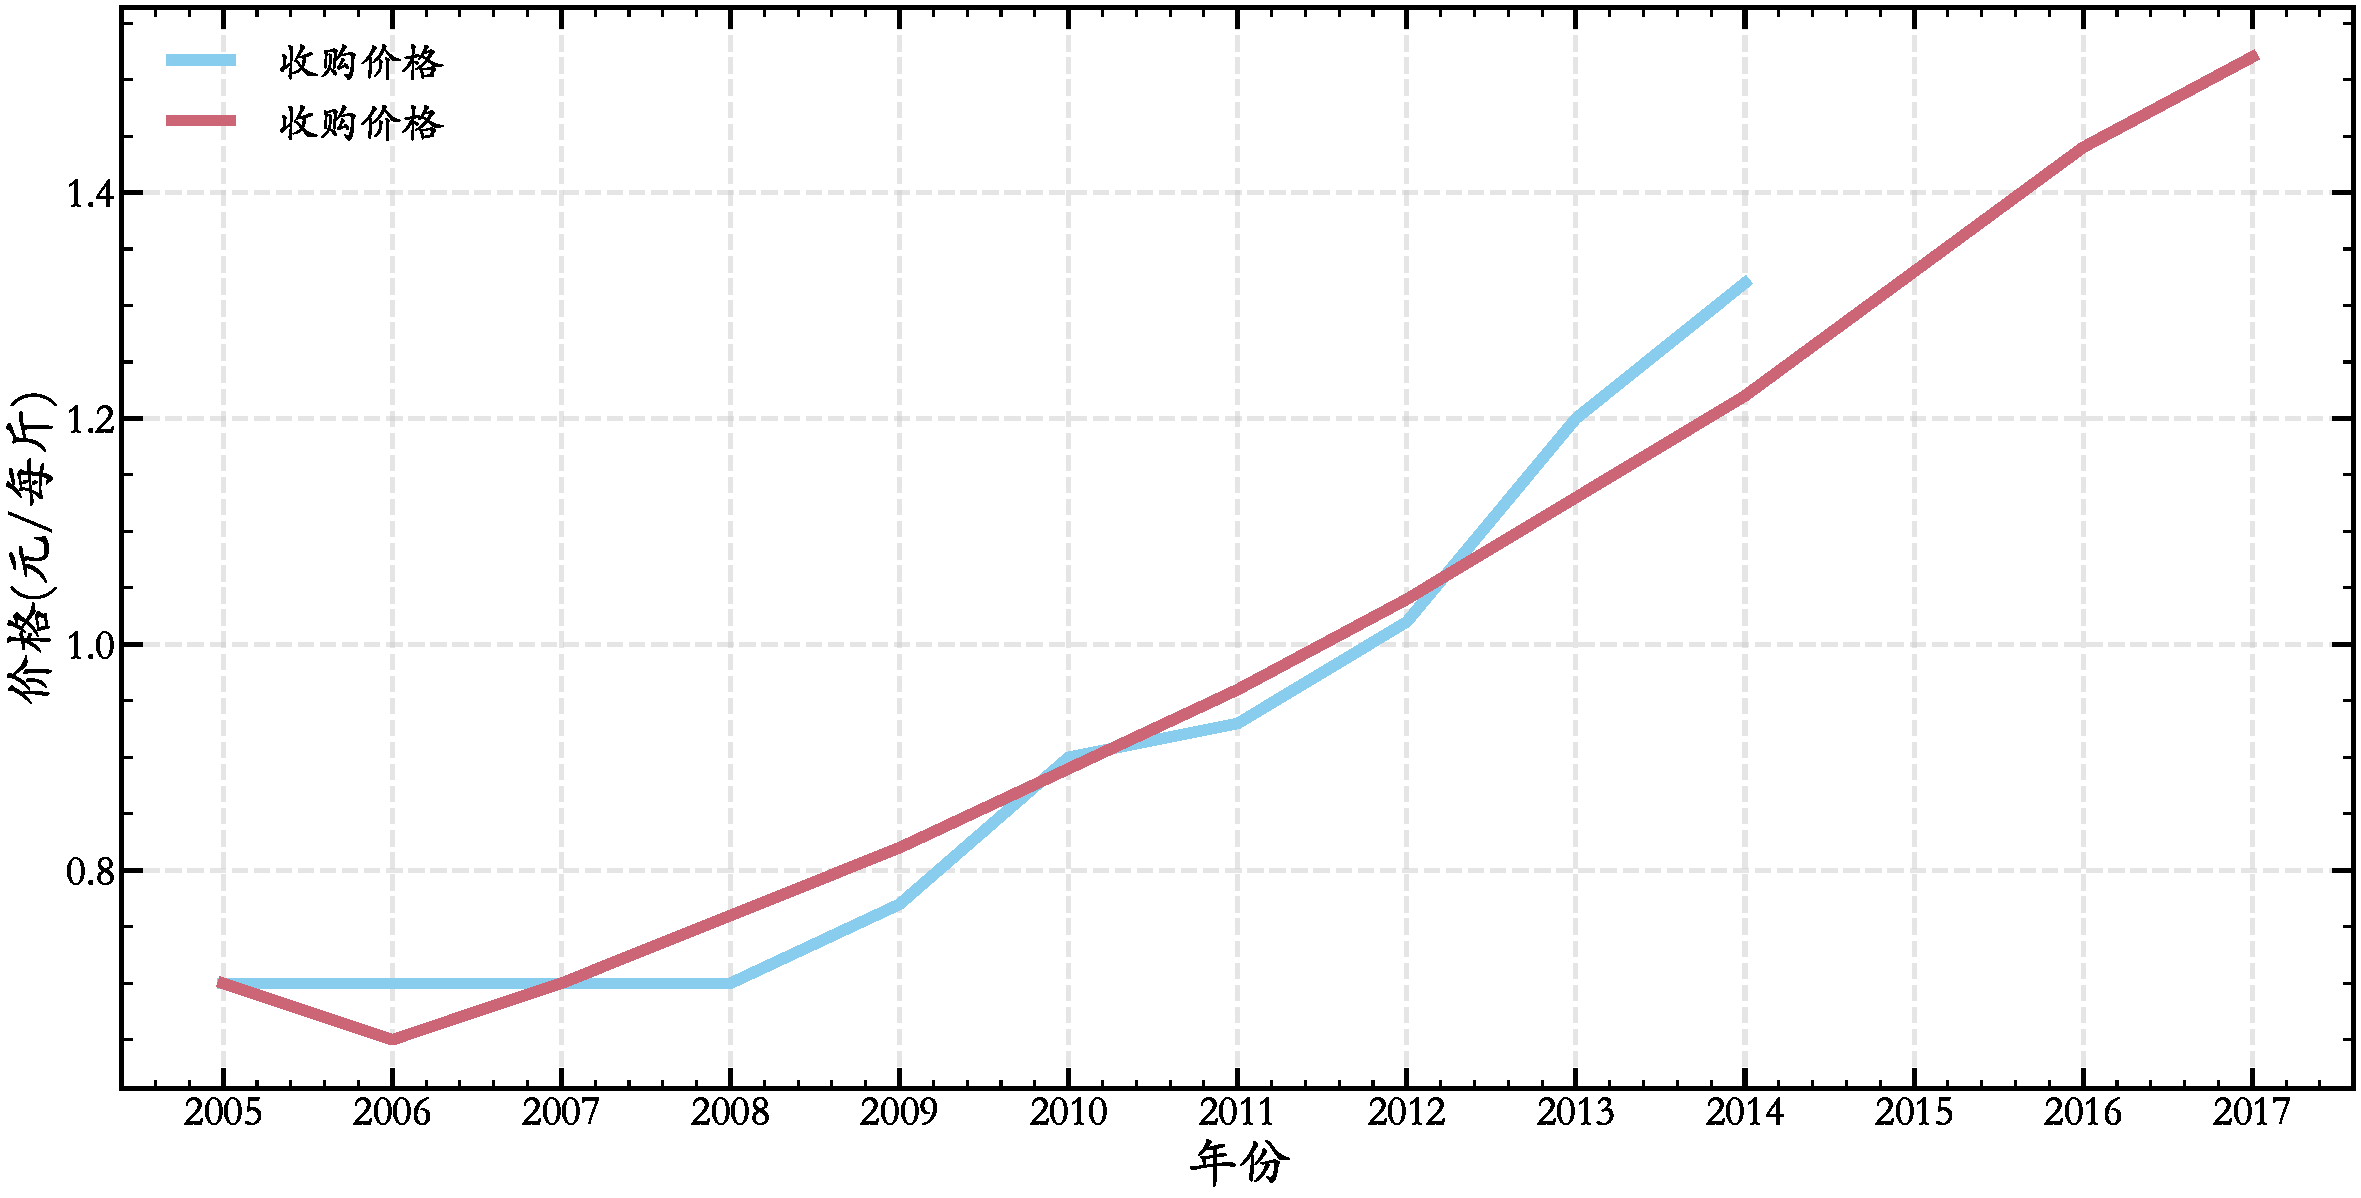
\includegraphics[width=0.935\textwidth]{fig3.pdf}
    \caption{最低收购价预测}
    \label{fig:gm}
\end{figure}\par
\section{问题五:粮食最低收购价的可行性分析}
假定国家想让水稻种植面积增加5\%,可以通过调整最低收购价来实现。为此,需对问题四中水稻最低收购价格的合理定价模型进行调整,调整后的水稻最低收购价格的合理定价模型只需对目标函数进行修改:
\begin{gather}
max PR_{t}=-\frac{1}{(1+5\%)\lambda_{5}}(-G_{t}^{s}+\lambda_{0}+\lambda_{1}G_{t-1}^{s}+\lambda_{2}P_{t-1}+\lambda_{3}IM_{t}+\lambda_{4}UP_{t})\notag
\end{gather}
运用Matlab,对上述水稻最低收购价格的合理定价模型进行运算,可以得到水稻合理最低收购价,即可以通过调整水稻最低收购价来实现水稻种植面积增加5\%的问题。依据Matlab计算结果得出,当水稻种植面积提高5\%后,水稻最低收购价格为153元。

\section{问题六:粮食种植的决策和建议}
\subsection{从影响粮食种植面积因素方面}
由问题一的研究结论可得,粮食种植面积受多种因素的影响,并且粮食种植区域的不同对于粮食种植面积的影响因素也是不同的。因此,若想提高粮食种植面积扩大粮食产量,应该根据其地域的不同,找出对粮食种植面积具有显著性影响的因素,制定相应的政策措施。\par
对于水稻来说,在其主产区湖南省与种植面积相关的因素有农村劳动力人口、城乡收入差距,水稻市场价格、水稻成本、总播种面积、受灾情况,但对其具有显著性为总播种面积和水稻市场价格,因此调控湖南省种植面积要注重调整这两个因素对种植面积的影响。国家和政府在以后制定关于粮食的相关政策时要对症下药,因地制宜。
\subsection{从粮食最低收购价政策实施方面}
问题二的研究看出,粮食最低收购价政策的实施对于不同区域的影响效果是不同的。并且不是所有粮食生产省份实施粮食最低收购价对粮食种植面积有积极影响,发现政策对辽宁省水稻种植面积有积极影响,对湖南省水稻种植面积影响不大。因此,在实施粮食最低收购政策时,要因地域的不同而制定不同的最低收购价政策或补贴政策。
\subsection{从粮食价格规律方面}
由问题三的研究可得,粮食供给、价格和需求分别受不同外生变量的影响,同时它 们三者之间又是相互影响、相互制约、共同演化的动态关系。要平衡粮食供需并稳定粮 食价格,需要权衡各方面的因素。粮食供给增长最大的一个原因是生产者对预期价格的 高估,造成粮食总量供给相对过剩,因此有关部门要打造粮食价格信息咨询平台,引导 生产者对粮食价格进行合理的预期进而进行合理的种植决策。
\subsection{从粮食最低收购价制定方面}
最低收购价并不是实际的市场收购价格,是收购粮食的底价。粮农决定是否种植 粮食,取决于很多因素,但最主要的还是看种植粮食所获得的纯收益的大小。粮食最低 收购价的公布,使得粮农能清楚地算出这笔经济账。因此粮食最低收购价的高低直接影 响着当年的粮食生产。过高的粮食最低收购价不仅会提高粮食市场价格从而加重消费者 负担,同时也会增加粮食的库存压力和国家财政的支出风险。另一方面,过低的粮食最 低收购价会打压粮农种植粮食的积极性,造成粮食种植面积的萎缩,这更不是国家所愿 意看到的。国家要积极调整粮食最低收购价既不能损害消费者分利益也不能使粮农受到 损失。经过问题四、五的研究,在合理的粮食最低收购价范围内,我们可以通过适当的 调整粮食最低收购价来调控粮食种植面积。



		\section{模型的评价}
		\subsection{模型评价}
		\subsubsection{优点:}\par
		\begin{enumerate}
		\item 本文在第一题中采用的斯皮尔曼(Spearman)相关系数对数据不要求服从正态分布,并且可以反映变量之间的趋同关系。
		\item 本文在第二题中运用主成分回归消除变量之间的共线性,同时在第三题中运用主成分-统计控制模型,消除协变量对水稻种植面积的影响,结果科学可信。
		\item 我们运用matlab,stata,python,结果相对科学且可视化程度高。
		\end{enumerate}
		\subsubsection{缺点:}\par
		\begin{enumerate}
		\item 基于前提假设进行研究,可能有些与实际情况不符。
		\item 供需及价格联动模型只能对粮食进行中短期预测,长期预测误差较大。
		\end{enumerate}

		
		

\bibliography{book.bib}
\newpage%附录新起一页
\begin{appendices}		
	\section{matlab 源代码}
	\begin{matlab}
	clc,clear
	a=xlsread('liaoning.xlsx'); 
	a=a(:,1:end-1);
	[m,n]=size(a);
	x0=a(:,[2:end]); y0=a(:,1); 
	hg1=[ones(m,1),x0]\y0; 
	hg1=hg1' 
	fprintf('y=%f',hg1(1)); 
	for i=2:n
	    if hg1(i)>0  
	       fprintf('+%f*x%d',hg1(i),i-1);
	    else
	       fprintf('%f*x%d',hg1(i),i-1)
	    end
	end
	fprintf('\n')  
	r=corrcoef(x0)  
	xd=zscore(x0);  
	yd=zscore(y0);  
	[vec1,lamda,rate]=pcacov(r)
	f=repmat(sign(sum(vec1)),size(vec1,1),1); 
	vec2=vec1.*f 
	contr=cumsum(rate) 
	df=xd*vec2;  
	num=input('请选项主成分的个数:')   
	hg21=df(:,[1:num])\yd  
	hg22=vec2(:,1:num)*hg21  
	hg23=[mean(y0)-std(y0)*mean(x0)./std(x0)*hg22, std(y0)*hg22'./std(x0)]  
	fprintf('y=%f',hg23(1)); 
	for i=2:n
	    if hg23(i)>0
	        fprintf('+%f*x%d',hg23(i),i-1);
	    else
	        fprintf('%f*x%d',hg23(i),i-1);
	    end
	end
	fprintf('\n')
	rmse2=sqrt(sum((hg23(1)+x0*hg23(2:end)'-y0).^2)/(m-num)) 
	\end{matlab}
	
	\begin{matlab}
	clc,clear all;
	B=xlsread('b.xlsx','B2:B20');
	lamada=B(1:6);beta=B(7:13);alpha=B(14:19);
	data=xlsread('3.xls','B18:L21');
	for i=1:4
	    f=[-1/lamada(5),0,0,0];
	    A=[1/lamada(5),0,0,0;
	        0,0.9,0,-1];
	    b1=(lamada(6)+lamada(1)*data(i,5)+lamada(2)*data(i,1)+lamada(3)*data(i,6)...
	    +lamada(4)*data(i,2))/lamada(5);
	    b=[31765+b1;0];
	    Aeq=[-beta(1),1,0,-beta(6);
	        0,-alpha(1),1,0];
	    beq1=beta(7)+beta(2)*data(i,1)+beta(3)*data(i,8)+beta(4)*data(i,9)+beta(5)*data(i,3);
	    beq2=alpha(6)+alpha(2)*data(i,10)+alpha(3)*data(i,3)+alpha(4)*data(i,9)+alpha(5)*data(i,11);
	    beq=[beq1;beq2];
	    lb=zeros(4,1);
	    %format bank
	    [x,fval,exitflag]=linprog(f,A,b,Aeq,beq,lb);
	    maz(i)=-fval+(lamada(6)+lamada(1)*data(i,5)+lamada(2)*data(i,1)+lamada(3)*data(i,6)...
	    +lamada(4)*data(i,2))/(-lamada(5));
	    price(i)=x(4)/15;
	    %maz(i)=-maz(i);
	end
	price
	\end{matlab}
	
	
	
	
	
	
	
	
	
	
	
	
	
	
	\section{python源代码}
	\begin{python}
	#encoding=gb2312
	import numpy as np
	import pandas as pd
	import seaborn as sns
	import matplotlib.pyplot as plt
	import palettable
	plt.rcParams['font.sans-serif']=['KaiTi']
	plt.rcParams['axes.unicode_minus']=False
	df = pd.read_excel('Spearmanliaoning.xlsx')
	print(df.columns)
	d=df.iloc[:,0:12]
	dcorr = d.corr(method='spearman')
	plt.figure(figsize=(15, 10),dpi=100)
	ax=sns.heatmap(data=dcorr,
	            vmax=0.3, 
	            cmap=palettable.cmocean.sequential.Tempo_20.mpl_colors[0:12],
	            annot=True,
	            fmt=".2f",
	            annot_kws={'size':8,'weight':'normal', 'color':'#253D24'},
	            square=True, linewidths=.5,
	            cbar_kws={"shrink": .5},
	            mask=abs(dcorr)<0.45,
	           )
	ax.set_xticklabels(ax.get_xticklabels(), rotation=-60)
	ax.set_yticklabels(ax.get_yticklabels(), rotation=60)
	ax.tick_params(axis='x',labelsize=11.7)
	ax.tick_params(axis='y',labelsize=11.7)  
	ax.xaxis.tick_top()
	plt.show()
	\end{python}
	
	
	\section{Stata源代码}
	\begin{python}
	ivregress y1 x5 x1 x6 x2 x7
	gmm (y1-{b1}*x5-{b2}*x1-{b3}*x6-b4*x2-{b5}*x7-{b6}),instruments (x5 x1 x6 x2 x7)
	
	\end{python}
	
	
	
	
	
	
	
	
	
	
	
	\section{SPSS交互命令}
	\begin{spss}
	NONPAR CORR 
	  /VARIABLES=水稻种植面积 农业劳动力人口 农民受教育程度 城乡收入差距 家庭负担 粳稻收购价 粳稻成本 相对竞争力 总播种面积 受灾情况 粮食的净出口 城市化水平 
	  /PRINT=SPEARMAN TWOTAIL NOSIG 
	  /MISSING=PAIRWISE.
	\end{spss}
	\begin{spss}
	FACTOR 
	  /VARIABLES 农民受教育程度 城乡收入差距 家庭负担 粳稻收购价 粳稻成本 总播种面积 城市化水平 
	  /MISSING LISTWISE 
	  /ANALYSIS 农民受教育程度 城乡收入差距 家庭负担 粳稻收购价 粳稻成本 总播种面积 城市化水平 
	  /PRINT INITIAL CORRELATION SIG EXTRACTION 
	  /CRITERIA FACTORS(3) ITERATE(25) 
	  /EXTRACTION PC 
	  /ROTATION NOROTATE 
	  /SAVE REG(ALL) 
	  /METHOD=CORRELATION.
	\end{spss}
	\begin{spss}
	REGRESSION 
	  /MISSING LISTWISE 
	  /STATISTICS COEFF OUTS R ANOVA COLLIN TOL 
	  /CRITERIA=PIN(.05) POUT(.10) 
	  /NOORIGIN 
	  /DEPENDENT 水稻种植面积 
	  /METHOD=ENTER FAC1_1 FAC2_1 FAC3_1.
	\end{spss}
\end{appendices}

\end{document}